\documentclass[12pt,fleqn]{article}

\usepackage{graphicx}
\usepackage{amsmath}
\usepackage{amssymb}
\usepackage{amsfonts}
\usepackage{amstext}
\usepackage{amsthm}
\usepackage{tikz}
%\setlength{\parindent}{2em}
\setlength{\parskip}{0ex}
\setlength{\oddsidemargin}{0in}
\setlength{\textwidth}{6.5in}
\setlength{\topmargin}{-.5in}
\setlength{\textheight}{9in}

\newcommand{\comment}[1]{}
\renewcommand{\thepage}{}

\begin{document}

%\renewcommand{\baselinestretch}{.95}

\setcounter{page}{1}
\thispagestyle{empty}

\begin{center}
\LARGE
CSE 211: Discrete Mathematics \\
Homework 2 \\
\normalsize 
\ \\
Fall 2018 \hfill assigned November 29, 2018 \\
Zafeirakis  Zafeirakopoulos, Instructor \hfill due December 10, 2018 \ \\
Ahmed Semih Ozmekik \hfill No$:171044039$

\end{center}

\normalsize

\begin{enumerate}


\item (5 points.) Prove that $B \subset A$ where
 
 $A = \{(a,b) \mid |a+b| < 21\}$ and
 $B = \{(a,b)\mid |a-1|<10 $ and $ |b-1| < 9\}$.
 \\\\
 $A = \{(a,b) \mid -21 < a+b < 21\}$  
 
 $B = \{(a,b)\mid -9 < a <11 $ $and $ $ -8 < b < 10\}$
 \\\\
 Rearrange $B$ :
 
 $B = \{(a,b)\mid (-9 < a <11) $ $+ $ $ (-8 < b < 10)\}$
 
 
 $B = \{(a,b)\mid (-17 < a + b < 21 )\}$\\
 
$A$ has every pair of $B$ has.(Not vice versa. $\therefore$ $ B \nsubseteq A $) $\therefore$ $ B \subset A $
 
 
 \item (10 points.) Write the expressions which represent the sets, given the Venn diagrams in Figure 1. 
 
\begin{figure}[h]
\centering
  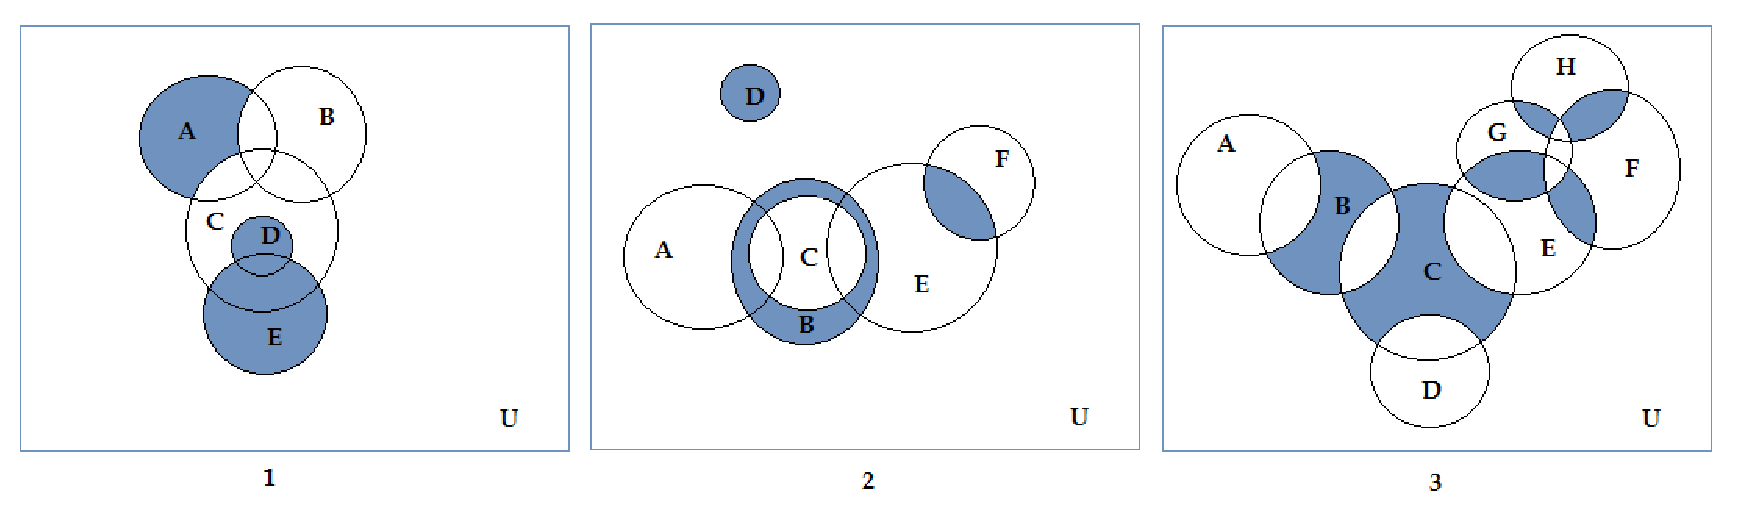
\includegraphics[width=150mm]{vennquestion.eps}
  \caption{}
  \label{}
\end{figure}

 1) $(A\setminus(B\cup C))\cup(D\cup E)$
 
 2) $(B\setminus C)\cup (F\cap E)\cup D$
 
 3) $(E\cap(G\cup F))\cup (H\cap (G\cup F))\setminus (G\cap F)\cup (B\setminus(A\cup C))\cup (C\setminus (B\cup E\cup D))$ 
 
 \item (10 points.) Let \(R\) be the relation on $\mathbb{R}^2$, defined by:

$(a_1, b_1)$ \(R\) $(a_2, b_2)$ if and only if either $a_1<a_2$ or both $a_1=a_2$
and $b_1\leq b_2$.

Prove that \(R\) is a partial order on  $\mathbb{R}^2$.

 	$R$ is Reflexive: for all $(a,b) \in \mathbb{R}^2$, we have $[(a,b),(a,b)]\in R$
    Since $a=a $ and $ b\leq b. $ 
    
    
   $R$ is Transitive: Whenever $[(a_1,b_1),(a_2, b_2)]\in R $ and $ [(a_2,b_2),(a_3, b_3)]\in R, $ we have $ [(a_1,b_1),(a_3,b_3)]\in R. $ Since, if $ a_1<a_2 $ and $ a_2<a_3 $, therefore $ a_1<a_3 $ holds; or if $ a_1=a_2 $ and $ b_1\leq b_2 $, $ a_2 = a_3 $ and $ b_2\leq b_3 $, therefore $ a_1 = a_3 $ and $ b_1\leq b_3 $ holds.     
    
       
    $R$ is Antisymmetric: Whenever $(a_1,b_1)\neq (a_2,b_2)$ and $[(a_1,b_1),(a_2, b_2)]\in R $, we have $[(a_2,b_2),(a_1, b_1)] \notin R $. Since, if $ a_1<a_2 $, then $a_2 \nless a_1 $, so there is no such element. Or, when $ a_1=a_2 $ and $ b_1\leq b_2 $, if $ a_2 = a_1 $ and $ b_2\leq b_1 $. Therefore $ a_2 = a_1 $ and $b_2 = b_1 $, $(a_1,b_1) =  (a_2,b_2)$. Which conflicts with our assumption, therefore $[(a_2,b_2),(a_1, b_1)] \notin R $. 
 	

\item (15 points.) Let  a partial order relation \(R\) on $X=\{n\in \mathbb{Z} : 2 \leq n \leq 12 \}$, defined by:

$x R y$  if and only if either (\(x\) is prime and $x < y$) or (\(x\) divides \(y\)).

Draw a Hasse diagram for \(R\), and identify the least element and the maximal elements.\\\\


\begin{tikzpicture}
    \begin{tikzpicture}
   	% Again:
   	\node (two) at (0,0) {$2$};
   	\node [above of=two] (three) {$3$};
   	\node [left of=three] (four) {$4$};
   	\node [above of=three] (five) {$5$};
   	\node [above left of=five] (six) {$6$};
   	\node [above of=five] (seven) {$7$};
   	\node [above left of=six] (eight) {$8$};
   	\node [above of=seven] (eleven) {$11$};
   	\node [right of=eleven] (nine) {$9$};
	\node [above of=eleven] (twelve)  {$12$};
	\node [right of=nine] (ten) {$10$}; 
   
	\draw [black,  thick, shorten <=-2pt, shorten >=-2pt] (two) -- (three);
	\draw [black,  thick, shorten <=-2pt, shorten >=-2pt] (three) -- (five);
	\draw [black,  thick, shorten <=-2pt, shorten >=-2pt] (five) -- (seven);  
	\draw [black,  thick, shorten <=-2pt, shorten >=-2pt] (eleven) -- (seven);
	\draw [black,  thick, shorten <=-2pt, shorten >=-2pt] (nine) -- (seven);
	\draw [black,  thick, shorten <=-2pt, shorten >=-2pt] (five) -- (six);
	\draw [black,  thick, shorten <=-2pt, shorten >=-2pt] (two) -- (four);
	\draw [black,  thick, shorten <=-2pt, shorten >=-2pt] (four) -- (eight);
	\draw [black,  thick, shorten <=-2pt, shorten >=-2pt] (twelve) -- (six);
	\draw [black,  thick, shorten <=-2pt, shorten >=-2pt] (eleven) -- (twelve);
	\draw [black,  thick, shorten <=-2pt, shorten >=-2pt] (eight) -- (seven);
	\draw [black,  thick, shorten <=-2pt, shorten >=-2pt] (ten) -- (seven);   
    
    
    
\end{tikzpicture}
\end{tikzpicture}


Maximal Elements: $12,9,10,8$

Least Element: $2$


\item (10 points.) Examine all Boolean lattices with cardinalities \(1-5\). Explain these lattice structures in detail.

\item (10 points.) Determine whether each of the following functions is injective, surjective, both or neither.

\begin{enumerate}
\item $f:\mathbb{Z}\rightarrow\mathbb{Z}, f(n)=n+(-1)^n$
\item $f:\mathbb{R}\rightarrow\mathbb{R}, f(n)=2^x$
\item $f:\mathbb{R}\rightarrow\mathbb{R}^+ \cup \{0\}, f(n)=x+|x|$
\end{enumerate}

\begin{enumerate}
\item Let $x ,y,k,l \in \mathbb{Z}$
      
 Every image has preimage. It is surjective.     
      
 Say $x=2k $ and $y=2l. $ $ x+1 = y+1 \therefore x=y. $
 
 Say $x=2k+1 $ and  $y=2l+1. $  $ x-1 = y-1 \therefore x=y. $ It is injective. 
 
\item Let $x , y \in \mathbb{R}$

 There is no image $x$ such that $ f(x)=0. $ It is not surjective.
 
 $2^x = 2^y \therefore x=y   $  It is injective.
  
\item Let $x , y \in \mathbb{R}$
 
 Every image has a preimage. It is surjective. 
 
 If $x,y < 0$ then, $f(x) = f(y) = 0. $ It is not injective.

\end{enumerate}

\item (15 points.) Let $f:X \rightarrow Y$ be a function. 

Show that function $  f  $ is bijective if and only if $f(X-Z)=Y-f(Z)$, for every subset \(Z\) of \(X\).

Let $X = X+Z$ \\
$f(X+Z-Z)=f(X)+f(Z)-f(Z)$\\
$f(X)=f(X)$\\
$\therefore f$ is bijective.

\item (15 points.) Let \(S\) denote the set of real $2 \times 2$ matrices of the form
$\begin{pmatrix} 
 a & b \\
-b & a 
\end{pmatrix}$

where \(a\) and \(b\) are not both zero. Show that \(S\) is a group under the operation of matrix multiplication.\\

To be able to be a group, one must satisfy these things: 
\begin{enumerate}
\item Must be closed under the operation .
\item Must be Associativitive.
\item Must have identity element.
\item Must have inverse element.
\end{enumerate}
Proofs has ben made due to this order, in below.

\begin{enumerate}


\item It is closed, under operation of matrix multiplication.
$a,b \in \mathbb{R}.$ Thus, $ a^2 + b^2 \in \mathbb{R}.$ 
\item 

$\begin{pmatrix} 
 1 & 2 \\
-2 & 1 
\end{pmatrix}\times (\begin{pmatrix} 
 3 & 4 \\
-4 & 3 
\end{pmatrix} \times \begin{pmatrix} 
 5 & 1 \\
-1 & 5 
\end{pmatrix}) = (\begin{pmatrix} 
 1 & 2 \\
-2 & 1 
\end{pmatrix}\times \begin{pmatrix} 
 3 & 4 \\
-4 & 3 
\end{pmatrix}) \times \begin{pmatrix} 
 5 & 1 \\
-1 & 5 
\end{pmatrix} $ 

\item
$\begin{pmatrix} 
 1 & 0 \\
 0 & 1 
\end{pmatrix} $

\item
An element exists in that group such that, $a,b \in \mathbb{R}.$ \\
Thus, $ a^2 + b^2 \in \mathbb{R} $ and $\frac{1}{a^2 + b^2 } $ $\in \mathbb{R}.$\\
($\frac{1}{a^2 + b^2 } $ is the inverse element.)



\end{enumerate}


\item (10 points.) Define the ring $\mathbb{Z}_n$. Show that $\mathbb{Z}_n$ is a field if and only if \(n\) is a prime number.

A ring is a set $S$ with two defined binary operators satisfying the following conditions:
\begin{enumerate}
\item Additive associativity.
\item Additive commutativity.
\item Additive identity.
\item Additive inverse.
\item Left and right distributivity.
\item Multiplicative associativity.
\end{enumerate}

For a ring to be a field, also four operations must be defined.



n=5 case:(n is a prime number)

    \begin{tabular}{|r|r|r|r|r|}
    \hline
     & 1 & 2 & 3 & 4\\
    \hline
    1 & 1 & 2 & 3 & 4\\
    \hline
    2 & 2 & 4 & 1 & 3\\
    \hline
    3 & 3 & 1 & 4 & 2\\
    \hline
    4 & 4 & 3 & 2 & 1\\
    \hline
    \end{tabular}

n=6 case:(n is not a prime number)
      
    \begin{tabular}{|r|r|r|r|r|r|}
    \hline
     & 1 & 2 & 3 & 4 & 5\\
    \hline
    1 & 1 & 2 & 3 & 4 & 5\\
    \hline
    2 & 2 & 4 & 0 & 2 & 4\\
    \hline
    3 & 3 & 0 & 4 & 0 & 3\\
    \hline
    4 & 4 & 3 & 0 & 4 & 2\\
    \hline
    5 & 5 & 4 & 3 & 2 & 1\\
    \hline
    \end{tabular}  

Some of the element has no inverse element.\\
$ \therefore $  This is not a field.
Besides, having $0$ in the table causing this ring not to become field anymore, since
this is against the identity element $1$.


\end{enumerate}

\end{document}
